
\documentclass{standalone}
\usepackage{xcolor}
\usepackage{pgfplots}
\pgfplotsset{compat=1.18}

\begin{document}

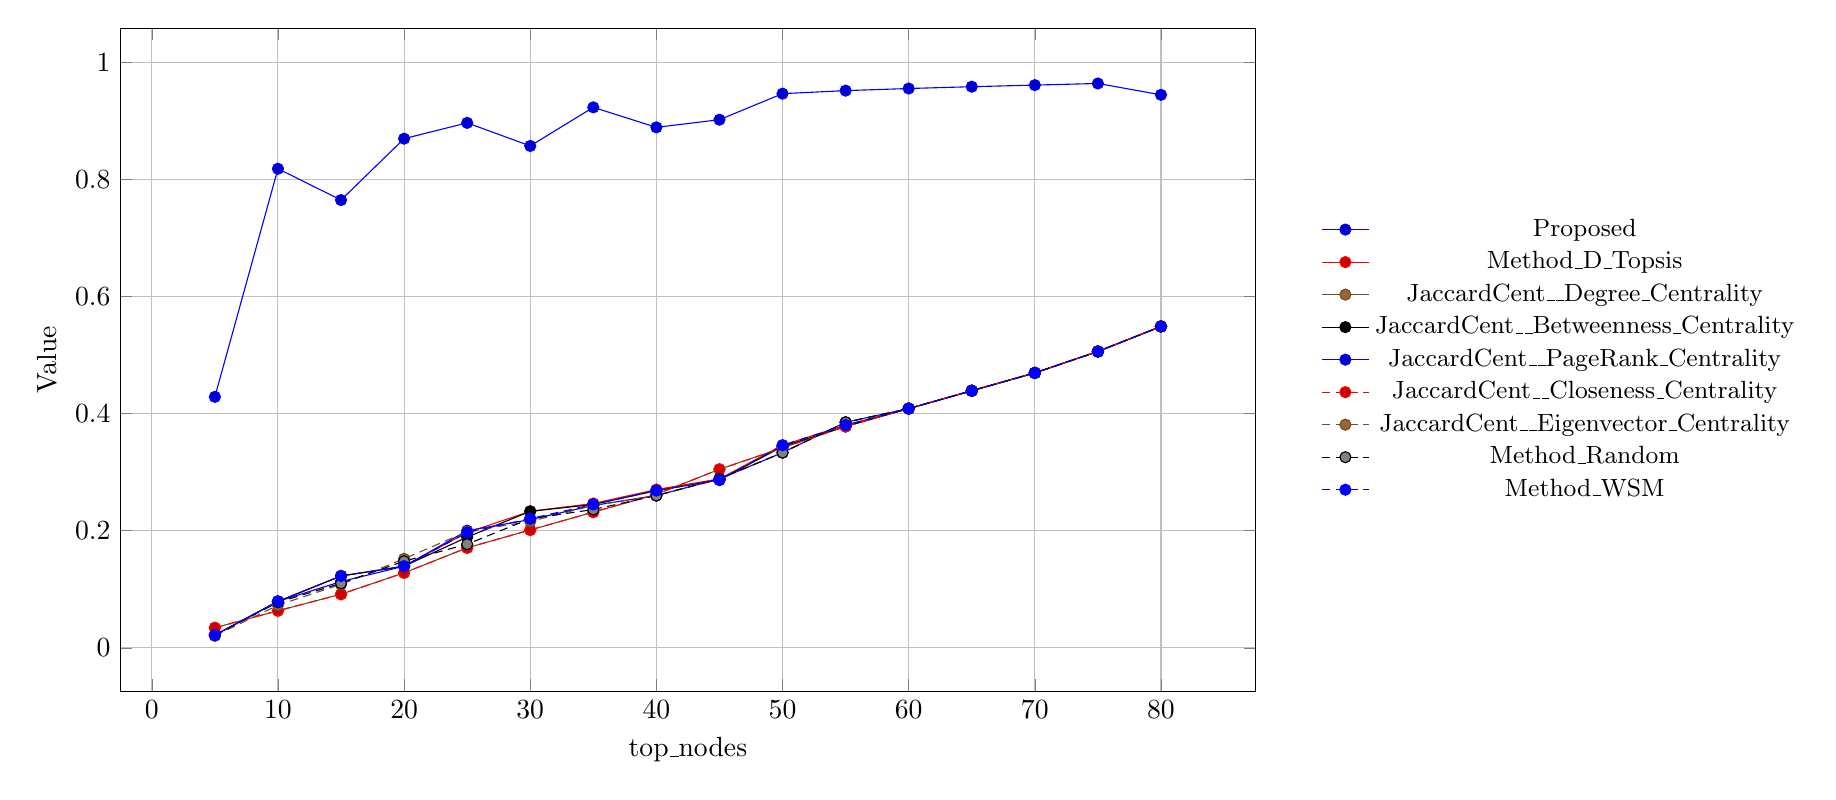
\begin{tikzpicture}
\begin{axis}[
    width=16cm,
    height=10cm,
    xlabel={top\_nodes},
    ylabel={Value},
    grid=major,
    legend style={
        at={(1.05,0.5)},
        anchor=west,
        font=\small,
        draw=none,
        cells={align=left},
    },
]
% Proposed
\addplot+[ mark=*] coordinates {
(5.0,0.4285714285714285) (10.0,0.8181818181818182) (15.0,0.7647058823529411) (20.0,0.8695652173913043) (25.0,0.896551724137931) (30.0,0.8571428571428571) (35.0,0.9230769230769232) (40.0,0.8888888888888888) (45.0,0.9019607843137256) (50.0,0.9464285714285714) (55.0,0.9516129032258064) (60.0,0.9552238805970148) (65.0,0.9583333333333334) (70.0,0.961038961038961) (75.0,0.963855421686747) (80.0,0.9444444444444444) };
\addlegendentry{Proposed}

% Method\_D\_Topsis
\addplot+[ mark=*] coordinates {
(5.0,0.0217391304347826) (10.0,0.0792079207920792) (15.0,0.1226415094339622) (20.0,0.1393442622950819) (25.0,0.1968503937007874) (30.0,0.2330827067669172) (35.0,0.2464788732394366) (40.0,0.2702702702702703) (45.0,0.2884615384615384) (50.0,0.3459119496855345) (55.0,0.3803680981595092) (60.0,0.4085365853658536) (65.0,0.4390243902439024) (70.0,0.4695121951219512) (75.0,0.5060975609756098) (80.0,0.5487804878048781) };
\addlegendentry{Method\_D\_Topsis}

% JaccardCent\_\_Degree\_Centrality
\addplot+[ mark=*] coordinates {
(5.0,0.0342465753424657) (10.0,0.0632911392405063) (15.0,0.0914634146341463) (20.0,0.1280487804878048) (25.0,0.1707317073170731) (30.0,0.2012195121951219) (35.0,0.2317073170731707) (40.0,0.2621951219512195) (45.0,0.3048780487804878) (50.0,0.3414634146341463) (55.0,0.3780487804878049) (60.0,0.4085365853658536) (65.0,0.4390243902439024) (70.0,0.4695121951219512) (75.0,0.5060975609756098) (80.0,0.5487804878048781) };
\addlegendentry{JaccardCent\_\_Degree\_Centrality}

% JaccardCent\_\_Betweenness\_Centrality
\addplot+[ mark=*] coordinates {
(5.0,0.0217391304347826) (10.0,0.0792079207920792) (15.0,0.1226415094339622) (20.0,0.1393442622950819) (25.0,0.1889763779527559) (30.0,0.2330827067669172) (35.0,0.2447552447552447) (40.0,0.2684563758389262) (45.0,0.286624203821656) (50.0,0.34375) (55.0,0.3780487804878049) (60.0,0.4085365853658536) (65.0,0.4390243902439024) (70.0,0.4695121951219512) (75.0,0.5060975609756098) (80.0,0.5487804878048781) };
\addlegendentry{JaccardCent\_\_Betweenness\_Centrality}

% JaccardCent\_\_PageRank\_Centrality
\addplot+[ mark=*] coordinates {
(5.0,0.0217391304347826) (10.0,0.0792079207920792) (15.0,0.1130434782608695) (20.0,0.1393442622950819) (25.0,0.2) (30.0,0.218978102189781) (35.0,0.2430555555555555) (40.0,0.26) (45.0,0.2884615384615384) (50.0,0.3333333333333333) (55.0,0.3850931677018633) (60.0,0.4085365853658536) (65.0,0.4390243902439024) (70.0,0.4695121951219512) (75.0,0.5060975609756098) (80.0,0.5487804878048781) };
\addlegendentry{JaccardCent\_\_PageRank\_Centrality}

% JaccardCent\_\_Closeness\_Centrality
\addplot+[ mark=*] coordinates {
(5.0,0.0342465753424657) (10.0,0.0632911392405063) (15.0,0.0914634146341463) (20.0,0.1280487804878048) (25.0,0.1707317073170731) (30.0,0.2012195121951219) (35.0,0.2317073170731707) (40.0,0.2621951219512195) (45.0,0.3048780487804878) (50.0,0.3414634146341463) (55.0,0.3780487804878049) (60.0,0.4085365853658536) (65.0,0.4390243902439024) (70.0,0.4695121951219512) (75.0,0.5060975609756098) (80.0,0.5487804878048781) };
\addlegendentry{JaccardCent\_\_Closeness\_Centrality}

% JaccardCent\_\_Eigenvector\_Centrality
\addplot+[mark=*] coordinates {
(5.0,0.0204081632653061) (10.0,0.0727272727272727) (15.0,0.1083333333333333) (20.0,0.152) (25.0,0.1984732824427481) (30.0,0.2158273381294964) (35.0,0.2430555555555555) (40.0,0.26) (45.0,0.2884615384615384) (50.0,0.3333333333333333) (55.0,0.3850931677018633) (60.0,0.4085365853658536) (65.0,0.4390243902439024) (70.0,0.4695121951219512) (75.0,0.5060975609756098) (80.0,0.5487804878048781) };
\addlegendentry{JaccardCent\_\_Eigenvector\_Centrality}

% Method\_Random
\addplot+[mark=*] coordinates {
(5.0,0.021505376344086) (10.0,0.0776699029126213) (15.0,0.110091743119266) (20.0,0.1478260869565217) (25.0,0.1769230769230769) (30.0,0.2205882352941176) (35.0,0.2361111111111111) (40.0,0.26) (45.0,0.2884615384615384) (50.0,0.3333333333333333) (55.0,0.3850931677018633) (60.0,0.4085365853658536) (65.0,0.4390243902439024) (70.0,0.4695121951219512) (75.0,0.5060975609756098) (80.0,0.5487804878048781) };
\addlegendentry{Method\_Random}

% Method\_WSM
\addplot+[ mark=*] coordinates {
(5.0,0.0217391304347826) (10.0,0.0792079207920792) (15.0,0.1226415094339622) (20.0,0.1393442622950819) (25.0,0.1968503937007874) (30.0,0.2205882352941176) (35.0,0.2447552447552447) (40.0,0.2684563758389262) (45.0,0.286624203821656) (50.0,0.3459119496855345) (55.0,0.3803680981595092) (60.0,0.4085365853658536) (65.0,0.4390243902439024) (70.0,0.4695121951219512) (75.0,0.5060975609756098) (80.0,0.5487804878048781) };
\addlegendentry{Method\_WSM}


\end{axis}
\end{tikzpicture}

\end{document}
